\documentclass{article}
\usepackage{amsmath}
\usepackage{tikz}
\usetikzlibrary{arrows.meta, positioning}

\begin{document}

\title{Problema de Transición de Rutas en Ingeniería Civil y Psicología}
\author{}
\date{}
\maketitle

\section*{Problema}

Un equipo de ingenieros civiles y psicólogos ambientales está investigando los patrones de movimiento de los peatones en un área urbana con cinco caminos alternativos. El objetivo del estudio es analizar las preferencias de las personas al elegir su ruta en función de distintas condiciones y estímulos externos, tales como señalización, tráfico y acceso a servicios, para mejorar la planificación urbana y promover rutas seguras y eficientes.

Cada día, un peatón que participa en el experimento comienza su recorrido en el mismo punto y puede elegir uno de cinco caminos: **A**, **B**, **C**, **D** o **E**. Las rutas se caracterizan de la siguiente manera:

\begin{itemize}
    \item \textbf{A}: Ruta directa pero ruidosa y poco amigable para peatones, sin áreas verdes.
    \item \textbf{B}: Ruta más larga pero con acceso a servicios (tiendas y cafés).
    \item \textbf{C}: Ruta rápida y silenciosa, con árboles y áreas verdes.
    \item \textbf{D}: Ruta con tráfico vehicular cercano y cruces no regulados.
    \item \textbf{E}: Ruta mixta con acceso a transporte público.
\end{itemize}

Al inicio del experimento, se observa que el peatón elige cada ruta con igual probabilidad. El comportamiento del peatón en función de la ruta elegida y la experiencia obtenida se observa durante un periodo de varios días. Las probabilidades de cambio de ruta al día siguiente, basadas en la experiencia del peatón, son las siguientes:

- Si el peatón elige la \textbf{Ruta A} y experimenta incomodidad por el ruido, la probabilidad de elegir la misma ruta al día siguiente es 0.3.
- Si el peatón elige la \textbf{Ruta B} y disfruta de los servicios, la probabilidad de elegir la misma ruta al día siguiente es 0.6.
- Si el peatón elige la \textbf{Ruta C} y encuentra un ambiente agradable, la probabilidad de repetir la misma ruta al día siguiente es 0.5.
- Si el peatón elige la \textbf{Ruta D} y enfrenta problemas de tráfico, la probabilidad de tomar la misma ruta al día siguiente es 0.2.
- Si el peatón elige la \textbf{Ruta E} y aprecia la conveniencia del transporte público, la probabilidad de elegir la misma ruta al día siguiente es 0.4.

\section*{Preguntas}

\begin{enumerate}
    \item (a) Escriba la matriz de transición para este proceso de Markov.
    \item (b) ¿Cuál es la probabilidad de que el peatón vuelva a elegir la Ruta A en el cuarto día (tercer día después del inicio del experimento)?
    \item (c) ¿Cuál es el vector de estado estacionario?
\end{enumerate}


El siguiente grafo ilustra las rutas y las probabilidades de que el peatón elija la misma o una ruta diferente al día siguiente:

\begin{center}
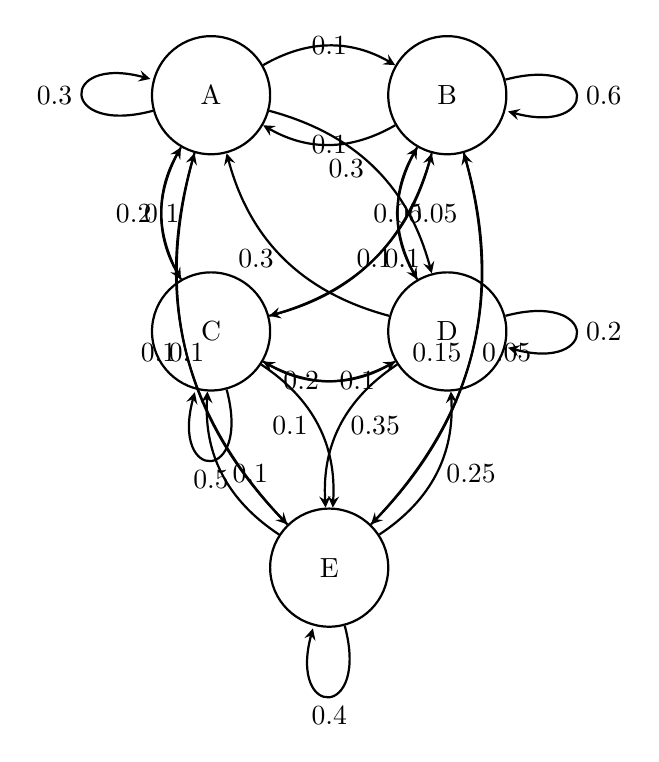
\begin{tikzpicture}[->, >=stealth, node distance=3cm, thick, main node/.style={circle, draw, minimum size=1.5cm}]
    
    % Nodes
    \node[main node] (A) {A};
    \node[main node] (B) [right of=A] {B};
    \node[main node] (C) [below of=A] {C};
    \node[main node] (D) [below of=B] {D};
    \node[main node] (E) [below of=C, xshift=1.5cm] {E};

    % Self-loops
    \path (A) edge[loop left] node {0.3} (A);
    \path (B) edge[loop right] node {0.6} (B);
    \path (C) edge[loop below] node {0.5} (C);
    \path (D) edge[loop right] node {0.2} (D);
    \path (E) edge[loop below] node {0.4} (E);

    % Arrows between nodes
    \path (A) edge[bend left] node {0.1} (B);
    \path (A) edge[bend right] node[left] {0.2} (C);
    \path (A) edge[bend left] node[left] {0.3} (D);
    \path (A) edge[bend right] node[left] {0.1} (E);

    \path (B) edge[bend left] node {0.1} (A);
    \path (B) edge[bend left] node {0.1} (C);
    \path (B) edge[bend right] node[right] {0.05} (D);
    \path (B) edge[bend left] node[right] {0.05} (E);

    \path (C) edge[bend left] node {0.1} (A);
    \path (C) edge[bend right] node[right] {0.1} (B);
    \path (C) edge[bend right] node[left] {0.2} (D);
    \path (C) edge[bend left] node[left] {0.1} (E);

    \path (D) edge[bend left] node[left] {0.3} (A);
    \path (D) edge[bend left] node {0.05} (B);
    \path (D) edge[bend left] node[right] {0.1} (C);
    \path (D) edge[bend right] node[right] {0.35} (E);

    \path (E) edge[bend left] node {0.1} (A);
    \path (E) edge[bend right] node[left] {0.15} (B);
    \path (E) edge[bend left] node[right] {0.1} (C);
    \path (E) edge[bend right] node[right] {0.25} (D);
    
\end{tikzpicture}
\end{center}

\end{document}
